\section{Versuch 3 - Auswertung der Motorgeschwindigkeit}
Der Motortreiber liefert ein analoges Spannungssignal, welches die aktuelle Motorgeschwindigkeit wiedergibt. Um die ADC-Werte in SI-Einheiten wird ein Polynom erster Ordnung benötigt. Hierfür werden mit Hilfe der ESCON-Studio konstante Motorgeschwindigkeiten ($\dot{\psi} \in \{ -3000, -2000,$  $-1000, 0, 1000, 2000, 3000 \} [rpm] $) gefahren und pro Durchlauf $m=500$ ADC-Werte aufgenommen. Über die Mittelwerte der Messungen und die vorgegebenen Radgeschwindigkeiten wird anschließend ein Polynom erster Ordnung approximiert.

\begin{figure}[h]
	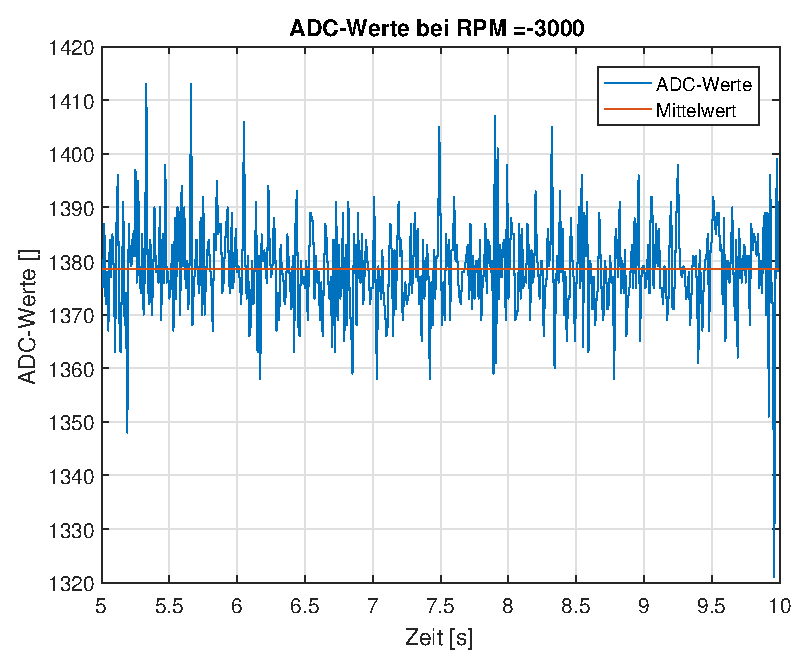
\includegraphics[width=0.5\linewidth]{img/adc_values_rpm_-3000.eps}
	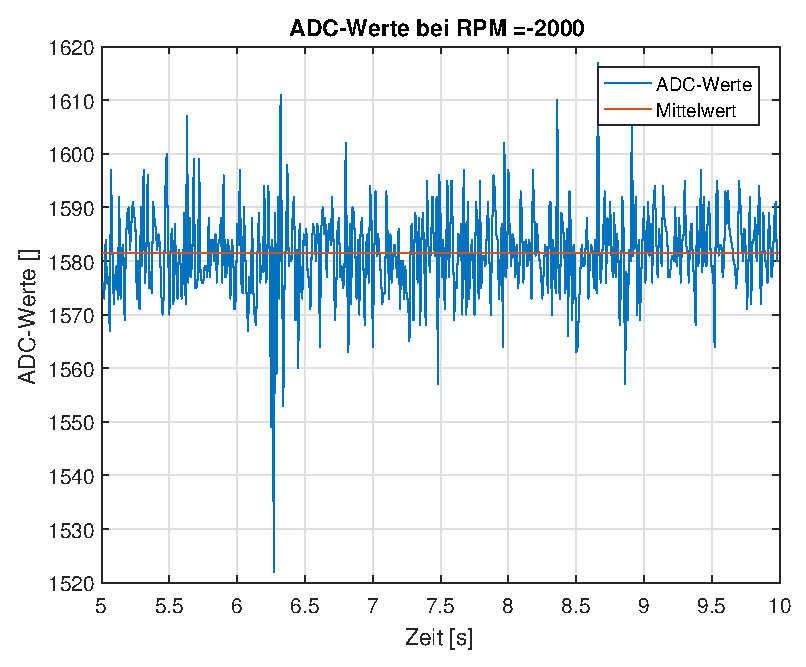
\includegraphics[width=0.5\linewidth]{img/adc_values_rpm_-2000.eps}
\end{figure}
\begin{figure}[h]
	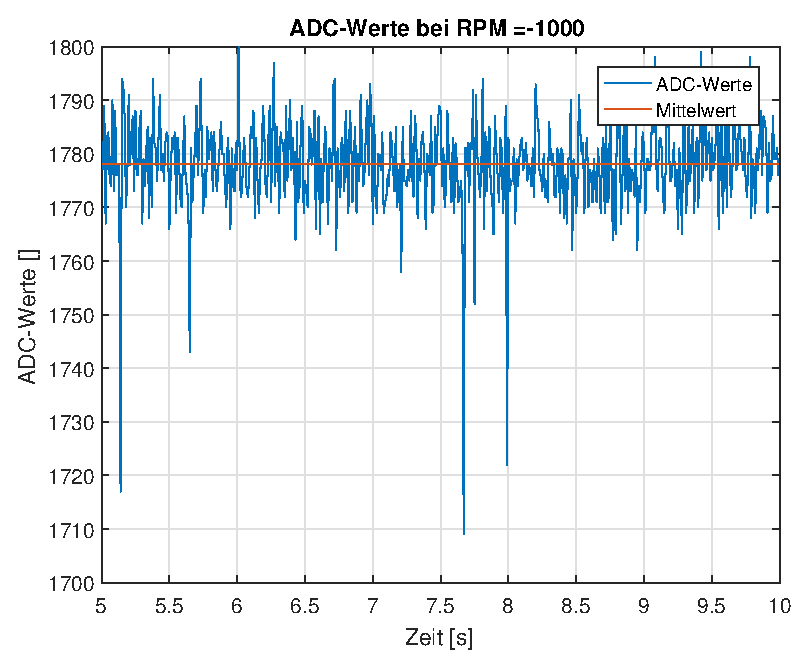
\includegraphics[width=0.5\linewidth]{img/adc_values_rpm_-1000.eps}
	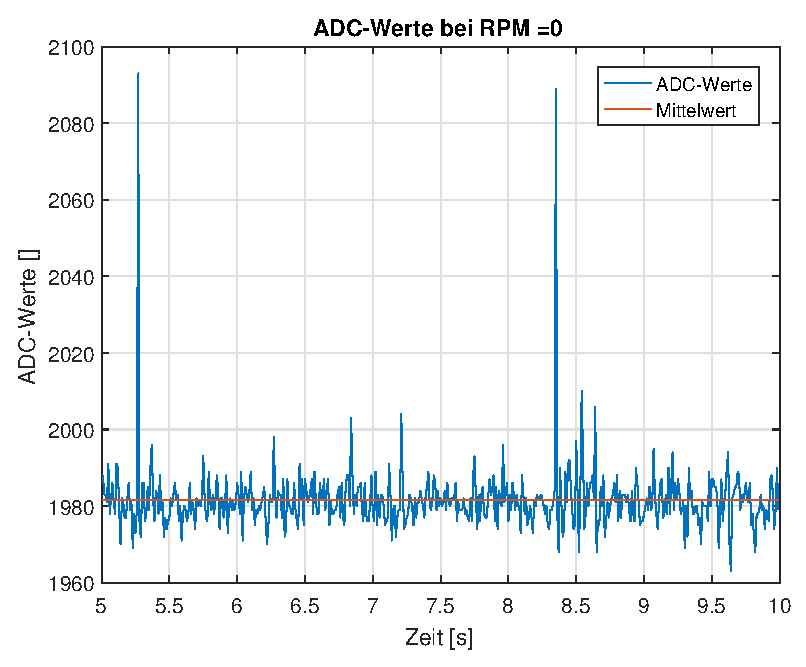
\includegraphics[width=0.5\linewidth]{img/adc_values_rpm_0.eps}
\end{figure}

\newpage
\begin{figure}[h]
	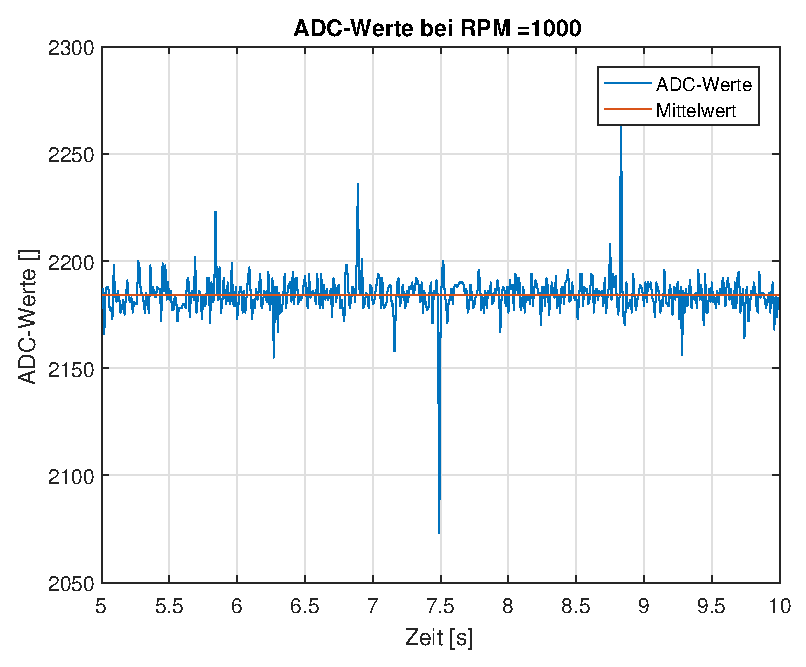
\includegraphics[width=0.5\linewidth]{img/adc_values_rpm_1000.eps}
	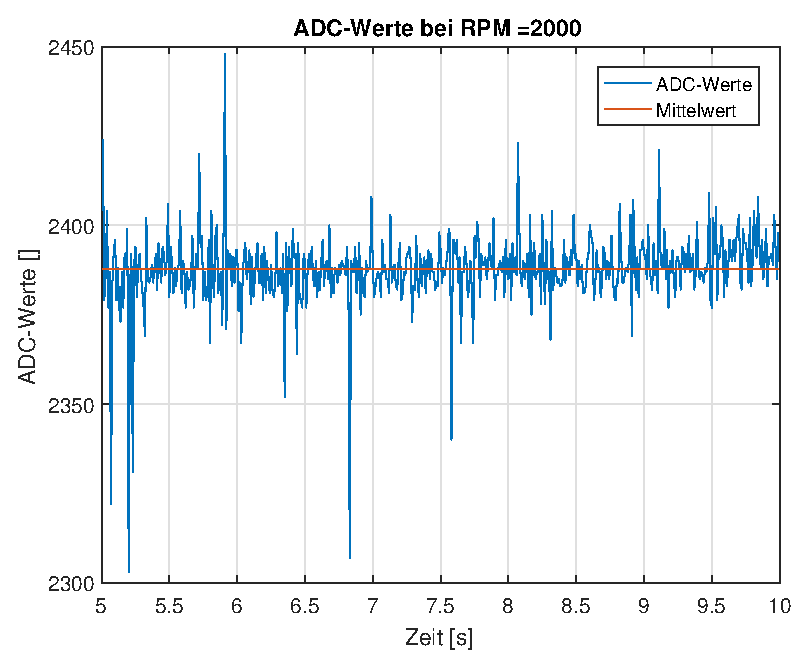
\includegraphics[width=0.5\linewidth]{img/adc_values_rpm_2000.eps}
\end{figure}
\begin{figure}[h]
\centering
	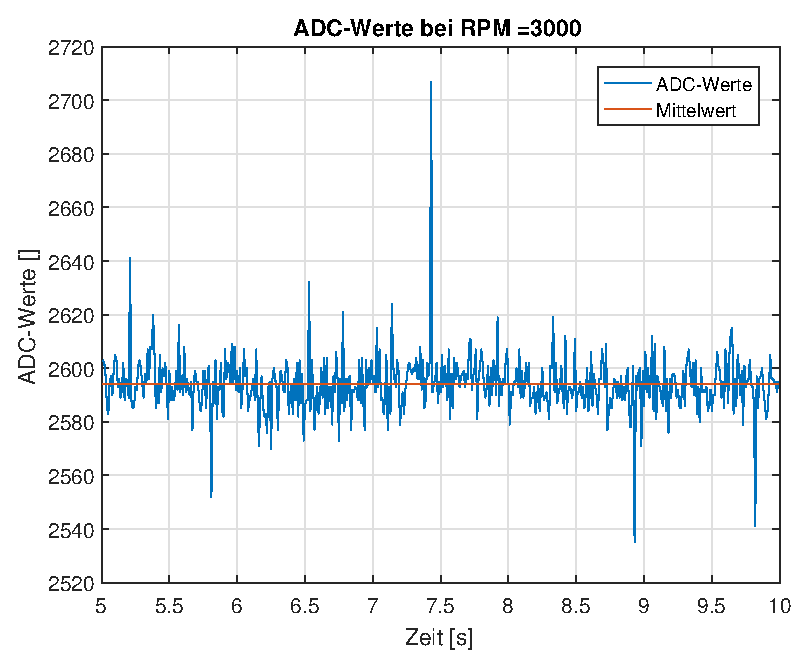
\includegraphics[width=0.5\linewidth]{img/adc_values_rpm_3000.eps}
\end{figure}

Mit Hilfe von MATLAB kann wird ein Polynom erster Ordnung berechnet, welches die ADC-Werte in SI-Einheiten umrechnet.

\begin{table}[h!]
\centering
\begin{tabular}{lcllcl}
$\dot{\psi}$ & $\equiv$ & Geschwindigkeit der Schwungmasse & $\dot{\psi}_{ADC}$ & $\equiv$ & ADC-Wert
\end{tabular}
\end{table}

\begin{equation}
\dot{\psi} = 0.5176 \cdot \dot{\psi}_{ADC} + -1017
\end{equation}

\begin{figure}[h!]
\centering
	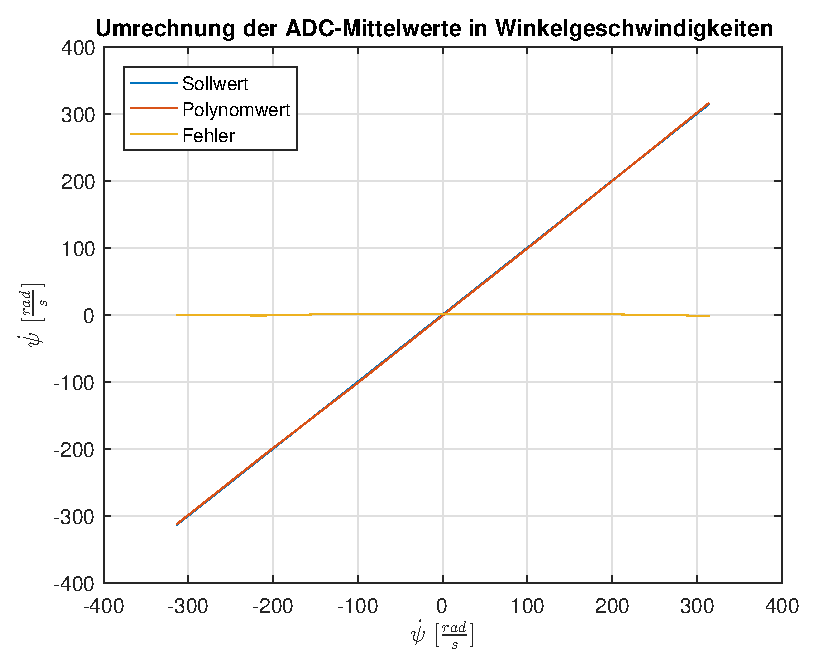
\includegraphics[width=0.5\linewidth]{img/ADC_mittelwert_polynom.eps}
\end{figure}